% debugging/debugging.tex

\QuickQuizChapter{chp:Validation}{Validation}

I have had a few parallel programs work the first time, but that is only
because I have written so many parallel programs over the past two decades.
And I have had far more parallel programs that fooled me into thinking
that they were working correctly the first time than actually were working
the first time.

I have therefore had great need of validation for my parallel programs.
The basic trick behind parallel validation, as with other software
validation, is to realize that the computer knows what is wrong.
It is therefore your job to force it to tell you.
This chapter can therefore be thought of as a short course in
machine interrogation.\footnote{
	But you can leave the thumbscrews and waterboards at home.
	This chapter covers much more sophisticated and effective
	methods, especially when you consider that most computer
	systems neither feel pain nor fear drowning.}

A longer course may be found in many recent books on validation, as
well as at least one rather old but quite worthwhile
one~\cite{GlenfordJMyers1979}.
Validation is an extremely important topic that cuts across all forms
of software, and is therefore worth intensive study in its own right.
However, this book is primarily about concurrency, so this chapter
will necessarily do little more than scratch the surface of this
critically important topic in Section~\ref{sec:debugging:Where Do Bugs Come From?}.

Section~\ref{sec:debugging:Required Mindset}
overviews the mindset required when validating software.
Section~\ref{sec:debugging:Tracing}
discusses tracing,
Section~\ref{sec:debugging:Assertions}
discusses assertions, and
Section~\ref{sec:debugging:Static Analysis}
discusses static analysis.
Section~\ref{sec:debugging:Code Review}
describes some unconventional approaches to code review that can
be helpful when the fabled 10,000 eyes are not looking at your code.
Section~\ref{sec:analysis:Probability and Heisenbugs}
gives an overview of the use of probability for validating parallel software.
More sections TBD.

\section{Where Do Bugs Come From?}
\label{sec:debugging:Where Do Bugs Come From?}

Bugs come from developers.
The basic problem is that the human brain did not evolve with computer
software in mind.
Instead, the human brain evolved in concert with other human brains and
with animal brains.
Because of this history, the following three characteristics of computers
often come as a shock to human intuition:

\begin{enumerate}
\item	Computers typically lack common sense, despite decades of research
	sacrificed at the alter of artificial intelligence.
\item	Computers generally fail to understand user intent, or more
	formally, computers generally lack a theory of mind.
\item	Computers usually do anything useful with a fragmentary plan,
	instead requiring that each and every detail of each and every
	possible scenario be spelled out in full.
\end{enumerate}

The first two points should be uncontroversial, as they are illustrated
by any number of failed products, perhaps most famously Clippy and
Microsoft Bob.
By attempting to relate to users as people, these two products raised
common-sense and theory-of-mind expectations that they proved incapable
of meeting.
Perhaps the set of software assistants that have recently started appearing
on smartphones will fare better.
That said, the developers working on them by all accounts still develop
the old way: the assistants might well benefit end users, but not so
much their own developers.

The human species's love of fragmentary plans deserves more explanation,
especially given that it is a classic two-edged sword.
This love of fragmentary plans is apparently due to the assumption that
the person carrying out the plan will have (1)~common sense and (2)~a good
understanding of the intent behind the plan.
This latter assumption is especially likely to hold in the common case
where the person doing the planning and the person carrying out the plan
are one and the same:  In this case, the plan will be revised almost
subconsciously as obstacles arise.
Therefore, the love of fragmentary plans has served human beings well,
in part because it is better to take random actions that have a high
probability of locating food than to starve to death while attempting
to plan the unplannable.
However, the past usefulness of fragmentary plans in everyday life is
no guarantee of their future usefulness in stored-program computers.

Furthermore, the need to follow fragmentary plans has had important effects
on the human psyche, due to the fact
that throughout much of human history, life was often difficult and dangerous.
It should come as no surprise that executing a fragmentary plan that had
a high probability of a violent encounter with sharp teeth and claws
requires almost insane levels of optimism---a level of optimism that actually
is present in most human beings.
In fact, the clinical term for a human being who lacks insane
levels of optimism is ``clinically depressed.'' Such people usually have
extreme difficulty functioning in their daily lives, underscoring the
perhaps counter-intuitive importance of insane levels of optimism to a
normal, healthy life.
If you are not insanely optimistic, you are less likely to start a difficult
but worthwhile project.\footnote{
	There are some famous exceptions to this rule of thumb.
	These are people who took on difficult but
	worthwhile projects in order to make at least a temporary escape
	from their depression.}

Important though insane levels of optimism might be, they are a key source
of bugs.
The question is therefore ``How to maintain the optimism required to start
a large project while at the same time injecting enough reality to keep
the bugs down to a dull roar?''
The next section examines the conundrum.

\section{Required Mindset}
\label{sec:debugging:Required Mindset}

When carrying out any validation effort, you should keep the following
defintions in mind:

\begin{enumerate}
\item	The only bug-free programs are trivial programs.
\item	A reliable program has no known bugs.
\end{enumerate}

From these definitions, it logically follows that any reliable
non-trivial program contains at least one bug that you do not
know about.
Therefore, any validation effort undertaken on a non-trivial program
that fails to find any bugs is itself a failure.
A good validation is therefore an exercise in destruction.
This means that if you are the type of person who enjoys breaking things,
validation is just the right type of job for you.

\QuickQuiz{}
	Suppose that you are writing a script that processes the
	output of the \co{time} command, which looks as follows:

	\vspace{5pt}
	\begin{minipage}[t]{\columnwidth}
	\tt
	\scriptsize
	\begin{verbatim}
		real    0m0.132s
		user    0m0.040s
		sys     0m0.008s
	\end{verbatim}
	\end{minipage}
	\vspace{5pt}

	The script is required to check its input for errors, and to
	give appropriate diagnostics if fed erroneous \co{time} output.
	What test inputs should you provide to this program to test it
	for use with \co{time} output generated by single-threaded programs?
\QuickQuizAnswer{
	\begin{enumerate}
	\item	Do you have a test case in which all the time is
		consumed in user mode by a CPU-bound program?
	\item	Do you have a test case in which all the time is
		consumed in system mode by a CPU-bound program?
	\item	Do you have a test case in which all three times
		are zero?
	\item	Do you have a test case in which the ``user'' and ``sys''
		times sum to more than the ``real'' time?
		(This would of course be completely legitimate in
		a multithreaded program.)
	\item	Do you have a set of tests cases in which one of the
		times uses more than one second?
	\item	Do you have a set of tests cases in which one of the
		times uses more than ten second?
	\item	Do you have a set of test cases in which one of the
		times has non-zero minutes?  (For example, ``15m36.342s''.)
	\item	Do you have a set of test cases in which one of the
		times has a seconds value of greater than 60?
	\item	Do you have a set of test cases in which one of the
		times overflows 32 bits of milliseconds?  64 bits of
		milliseconds?
	\item	Do you have a set of test cases in which one of the
		times is negative?
	\item	Do you have a set of test cases in which one of the
		times has a positive minutes value but a negative
		seconds value?
	\item	Do you have a set of test cases in which one of the
		times omits the ``m'' or the ``s''?
	\item	Do you have a set of test cases in which one of the
		times is non-numeric?  (For example, ``Go Fish''.)
	\item	Do you have a set of test cases in which one of the
		lines is omitted?  (For example, where there is a
		``real'' value and a ``sys'' value, but no ``user''
		value.)
	\item	Do you have a set of test cases where one of the
		lines is duplicated?  Or duplicated, but with a
		different time value for the duplicate?
	\item	Do you have a set of test cases where a given line
		has more than one time value?  (For example,
		``real 0m0.132s 0m0.008s''.)
	\item	Do you have a set of test cases containing random
		characters?
	\item	In all test cases involving invalid input, did you
		generate all permutations?
	\item	For each test case, do you have an expected outcome
		for that test?
	\end{enumerate}

	If you did not generate test data for a substantial number of
	the above cases, you will need to cultivate a more destructive
	attitude in order to have a chance of generating high-quality
	tests.

	Of course, one way to economize on destructiveness is to
	generate the tests with the to-be-tested source code at hand,
	which is called white-box testing (as opposed to black-box testing).
	However, this is no panacea: You will find that it is all too
	easy to find your thinking limited by what the program can handle,
	thus failing to generate truly destructive inputs.
} \QuickQuizEnd

But perhaps you are a super-programmer whose code is always perfect
the first time every time.
If so, congratulations!
Feel free to skip this chapter, but
I do hope that you will forgive my skepticism.
You see, I have met far more people who claimed to be able
to write perfect code the first time every time than I have
people who were actually capable of carrying out this feat.
And even if you really are a super-programmer, you just might
find yourself debugging lesser mortals' work.

One approach for the rest of us is to alternate between our normal
state of insane optimism
(Sure, I can program that!) and severe pessimism
(It seems to work, but I just know that there have to be more bugs hiding
in there somewhere!).
It helps if you enjoy breaking things.
If you don't, or if your joy in breaking things is limited to breaking
\emph{other} people's things, find someone who does love breaking your
code and get them to help you test it.

Another helpful frame of mind is to hate other people finding bugs in
your code.
This hatred can help motivate you to torture your code beyond reason
in order to increase the probability that you find the bugs rather than
someone else.

One final frame of mind is to consider the possibility that someone's
life depends on your code being correct.
This can also motivate you to torture your code into revealing the
whereabouts of its bugs.

This leaves the possibility of multiple people with different frames of
mind contributing to the project, with varying levels of optimism.
This can work well, if properly organized.

Other validation methodologies and techniques are covered in the following
sections, all of which are required to offset humanity's natural optimism.

\section{Tracing}
\label{sec:debugging:Tracing}

When all else fails, add a \co{printk()}!
Or a \co{printf()}, if you are working with user-mode C-language applications.

The rationale is simple: If you cannot figure out how execution reached
a given point in the code, sprinkle print statements earlier in the
code to work out what happened.
You can get a similar effect, and with more convenience and flexibility,
by using a debugger such as gdb (for user applications) or kgdb
(for debugging Linux kernels).
Much more sophisticated tools exist, with some of the more recent
offering the ability to rewind backwards in time from the point
of failure.

These brute-force testing tools are all valuable, especially now
that typical systems have more than 64K of memory and CPUs running
faster than 4MHz.
Much has been
written about these tools, so this chapter will add little more.

However, these tools all have a serious shortcoming when the job at hand
is to convince a the fastpath of a high-performance parallel algorithm
to tell you what is going wrong, namely, they often have excessive
overheads.
There are special tracing technologies for this purpose, which typically
leverage data ownership techniques
(see Chapter~\ref{chp:Data Ownership})
to minimize the overhead of runtime data collection.
One example within the Linux kernel is
``trace events''~\cite{StevenRostedt2010perfTraceEventP1,StevenRostedt2010perfTraceEventP2,StevenRostedt2010perfTraceEventP3,StevenRostedt2010perfHP+DeathlyMacros}.
Another example that handles userspace (but has not been accepted into
the Linux kernel) is LTTng~\cite{MathieuDesnoyers2009LFCollabSummit}.
Each of these uses per-CPU buffers to allow data to be collected with
extremely low overhead.

Tracing can be extremely useful, but it does have shortcomings.
For example, although the machine really does know all,
what it knows is almost always way more than your head can hold.
For this reason, high-quality test suites normally come with sophisticated
scripts to analyze the voluminous output.
But beware---scripts won't necessarily notice surprising things.
My rcutorture scripts are a case in point: Early versions of those
scripts were quite satisfied with a test run in which RCU grace periods
stalled indefinitely.
This of course resulted in the scripts being modified to detect RCU
grace-period stalls, but this does not change the fact that the scripts
will only detects problems that I think to make them detect.
The scripts are useful, but they are no substitute for me occasionally
scanning the rcutorture output.

Another problem with tracing and especially with \co{printk()} calls
is that their overhead is often too much for production use.
In some such cases, assertions can be helpful.

\section{Assertions}
\label{sec:debugging:Assertions}

Assertions are usually implemented in the following manner:

\vspace{5pt}
\begin{minipage}[t]{\columnwidth}
\tt
\scriptsize
\begin{verbatim}
  1 if (something_bad_is_happening())
  2   complain();
\end{verbatim}
\end{minipage}
\vspace{5pt}

This pattern is often encapsulated into C-preprocessor macros or
language intrinsics, for example, in the Linux kernel, this might
be represented as \co{WARN_ON(something_bad_is_happening())}.
Of course, if \co{something_bad_is_happening()} quite frequently,
the resulting output might obscure reports of other problems,
in which case
\co{WARN_ON_ONCE(something_bad_is_happening())} might be more appropriate.

\QuickQuiz{}
	How can you implement \co{WARN_ON_ONCE()}?
\QuickQuizAnswer{
	If you don't mind having a \co{WARN_ON_ONCE()} that
	will sometimes warn twice or three times, simply maintain
	a static variable that is initialized to zero.
	If the condition triggers, check the static variable, and
	if it is non-zero, return.
	Otherwise, set it to one, print the message, and return.

	If you really need the message to never appear more than once,
	perhaps because it is huge, you can use an atomic exchange
	operation in place of ``set it to one'' above.
	Print the message only if the atomic exchange operation returns
	zero.
} \QuickQuizEnd

In parallel code, one especially bad something that might happen is that
a function expecting to be called under a particular lock might be called
without that lock being held.
Such functions sometimes have header comments stating something like
``The caller must hold \co{foo_lock} when calling this function'', but
such a comment does no good unless someone actually reads it.
An executable statement like \co{lock_is_held(&foo_lock)} carries far
more force.

The Linux kernel's lockdep facility~\cite{JonathanCorbet2006lockdep}
takes this a step farther, reporting potential deadlocks as well as
allowing functions to verify that the proper locks are held.
Of course, this additional functionality incurs significant overhead,
so that lockdep is not necessarily appropriate for production use.

So what can be done in cases where checking is necessary, but where the
overhead of runtime checking cannot be tolerated?
One approach is static analysis, which is discussed in the next section.

\section{Static Analysis}
\label{sec:debugging:Static Analysis}

Static analysis is a validation technique were one program takes a second
program as input, reporting errors and vulnerabilities located in this
second program.
Interestingly enough, almost all programs are subjected to static analysis
by their compilers or interpreters.
These tools are of course far from perfect, but their ability to locate
errors has improved immensely over the past few decades, in part because
they now have much more than 64K bytes of memory in which to carry out their
analysis.

The sparse static analyzer.

\section{Code Review}
\label{sec:debugging:Code Review}

Various code-review activities are special cases of static analysis, but
with human beings doing the analysis.
This section covers inspection, walkthroughs, and self-inspection.

\subsection{Inspection}
\label{sec:debugging:Inspection}

Traditionally, formal code inspections take place in face-to-face meetings
with formally defined roles: moderator, developer, and one or two other
participants.
The developer reads through the code, explaining what it is doing and
why it works.
The one or two other participants ask questions and raise issues, while
the moderator's job is to resolve any conflicts and to take notes.
This process can be extremely effective at locating bugs, particularly
if all of the participants are familiar with the code at hand.

However, this face-to-face formal procedure does not necessarily
work well in the global Linux kernel community, although it might work
well via an IRC session.
Instead, individuals review code separately and provide comments via
email or IRC.
The note-taking is provided by email archives or IRC logs, and moderators
volunteer their services as appropriate.
Give or take the occasional flamewar, this process also works reasonably
well, particularly if all of the participants are familiar with the
code at hand.\footnote{
	That said, one advantage of the Linux kernel community approach
	over traditional formal inspections is the greater probability of
	contributions from people \emph{not} familiar with the code.}

It is quite likely that the Linux kernel community's review process
is ripe for improvement:

\begin{enumerate}
\item	There is sometimes a shortage of people with the time and
	expertise required to carry out an effective review.
\item	Even though all review discussions are archived, they are
	often ``lost'' in the sense that insights are forgotten and
	people often fail to look up the discussions.
	This can result in re-insertion of the same bugs.
\item	It is sometimes difficult to resolve flamewars when they do
	break out, especially when the combatants have disjoint
	goals, experience, and vocabulary.
\end{enumerate}

\subsection{Walkthroughs}
\label{sec:debugging:Walkthroughs}

A traditional code walkthrough is similar to a formal inspection,
except that the group
``plays computer'' with the code, driven by specific test cases.
A typical walkthrough team has a moderator, a secretary (who records
bugs found), a testing expert (who generates the test cases) and
perhaps one to two others.
These can be extremely effective, albeit also extremely time-consuming.

It has been some decades since I have participated in a formal
walkthrough, and I suspect that a present-day walkthrough would
use single-stepping debuggers.
One could imagine a particularly sadistic procedure as follows:

\begin{enumerate}
\item	The tester presents the test case.
\item	The moderator starts the code under a debugger, using the
	specified test case as input.
\item	Before each statement is executed, the developer is required
	to predict the outcome of the statement and explain why
	this outcome is correct.
\item	If the outcome differs from that predicted by the developer,
	this is taken as evidence of a potential bug.
\item	In parallel code, a ``concurrency shark'' asks what code
	might execute concurrently with this code, and why such
	concurrency is harmless.
\end{enumerate}

Sadistic, certainly.
Effective?
Maybe.
If the participants have a good understanding of the requirements,
software tools, data structures, and algorithms, then walkthroughs
can be extremely effective.
If not, they are often a waste of time.

\subsection{Self-Inspection}
\label{sec:debugging:Self-Inspection}

Although developers are usually not all that effective at inspecting
their own code, there are a number of situations where there is no
reasonable alternative.
For example, the developer might be the only person authorized to look
at the code, other qualified developers might all be too busy, or
the code in question might be sufficiently bizarre that the developer
is unable to convince anyone else to take is seriously until after
demonstrating a prototype.
In these cases, the following procedure can be quite helpful,
especially for complex parallel code:

\begin{enumerate}
\item	Write design document with requirements, diagrams for data structures,
	and rationale for design choices.
\item	Consult with experts, update the design document as needed.
\item	Write the code in pen on paper, correct errors as you go.
	Resist the temptation to refer to pre-existing nearly identical code
	sequences, instead, copy them.
\item	If there were errors, copy the code in pen on fresh paper, correcting
	errors as you go.
	Repeat until the last two copies are identical.
\item	Produce proofs of correctness for any non-obvious code.
\item	Where possible, test the code fragments from the bottom up.
\item	When all the code is integrated, do full-up functional and
	stress testing.
\item	Once the code passes all tests, write code-level documentation,
	perhaps as an extension to the design document discussed above.
\end{enumerate}

When I faithfully follow this procedure for new RCU code, there are
normally only a few bugs left at the end.
With some prominent exceptions~\cite{PaulEMcKenney2011RCU3.0trainwreck},
I usually manage to locate these bugs before others do.

\QuickQuiz{}
	Why would anyone bother copying existing code in pen on paper???
	Doesn't that just increase the probability of transcription errors?
\QuickQuizAnswer{
	If you are worried about transcription errors, please allow me
	to be the first to introduce you to a really cool tool named
	\co{diff}.
	In addition, carrying out the copying can be quite valuable:
	\begin{enumerate}
	\item	If you are copying a lot of code, you are probably failing
		to take advantage of an opportunity for abstraction.
		The act of copying code can provide great motivation
		for abstraction.
	\item	Copying the code gives you an opportunity to think about
		whether the code really works in its new setting.
		Is there some non-obvious constraint, such as the need
		to disable interrupts or to hold some lock?
	\item	Copying the code also gives you time to consider whether
		there is some better way to get the job done.
	\end{enumerate}
	So, yes, copy the code!
} \QuickQuizEnd

\QuickQuiz{}
	This procedure is ridiculously over-engineered!
	How can you expect to get a reasonable amount of software
	written doing it this way???
\QuickQuizAnswer{
	Indeed, repeatedly copying code by hand is laborious and slow.
	However, when combined with heavy-duty stress testing and
	proofs of correctness, this approach is also extremely effective
	for complex parallel code where ultimate performance and
	reliability are required and where debugging is difficult.
	The Linux-kernel RCU implementation is a case in point.

	On the other hand, if you are writing a simple single-threaded
	shell script to manipulate some data, then you would be
	best-served by a different methodology.
	For example, you might enter each command one at a time
	into an interactive shell with a test data set to make
	sure that it did what you wanted, then copy-and-paste the
	successful commands into your script.
	Finally, test the script as a whole.

	If you have a friend or colleague who is willing to help out,
	pair programming can work very well, as can any number of
	formal design- and code-review processes.

	And if you are writing code as a hobby, then do whatever you like.

	In short, different types of software need different development
	methodologies.
} \QuickQuizEnd

The above procedure works well for new code, but what if you need to
inspect code that you have already written?
You can of course apply the above procedure for old code in the special
case where you wrote one to throw away~\cite{Brooks79},
but the following approach can also be helpful in less desperate
circumstances:

\begin{enumerate}
\item	Using your favorite documentation tool (latex, html,
	OpenOffice, or straight ASCII), describe the high-level
	design of the code in question.
	Use lots of diagrams to illustrate the data structures
	and how these structures are updated.
\item	Make a copy of the code, stripping away all comments.
\item	Document what the code does statement by statement.
\item	Fix bugs as you find them.
\end{enumerate}

This works because describing the code in detail is an excellent way to spot
bugs~\cite{GlenfordJMyers1979}.
This second procedure is also a good way to get your head around someone
else's code, in fact, in many cases, the first step suffices.

Although review and inspection by others is probably more efficient and
effective, the above procedures can be quite helpful in cases where
for whatever reason it is not feasible to involve others.

At this point, you might be wondering how to write parallel code without
having to do all this boring paperwork.
Here are some time-tested ways of accomplishing this:

\begin{enumerate}
\item	Write a sequential program that scales through use of
	available parallel library functions.
\item	Write sequential plug-ins for a parallel framework,
	such as map-reduce, BOINC, or a web-application server.
\item	Do such a good job of parallel design that the problem
	is fully partitioned, then just implement sequential
	program(s) that run in parallel without communication.
\item	Stick to one of the application areas (such as linear algebra)
	where tools exist to automatically decompose and parallelize
	the problem.
\item	Make extremely disciplined use of parallel-programming
	primitives, so that it is easily seen to be correct.
	But beware: It is always tempting to break the rules
	``just a little bit'' to gain better performance or
	scalability.
	Breaking the rules often results in general breakage.
	That is, unless you carefully do the paperwork described in this
	section.
\end{enumerate}

But the sad fact is that even if you do the paperwork or use one of
the above ways to more-or-less safely avoid paperwork,
there will be bugs.
The next section describes how to handle the probabilistic bugs that
occur all too commonly when validating parallel software.

\section{Probability and Heisenbugs}
\label{sec:analysis:Probability and Heisenbugs}

So your parallel program fails.
Sometimes.

But you used techniques from the earlier sections to locate
the problem and now have a fix in place!
Congratulations!!!

Now the question is just how much testing is require in order to be
certain that
you actually fixed the bug, as opposed to just reducing the probability
of it occurring on the one hand, having fixed only one of several
related bugs on the other and, or made some ineffectual unrelated
change on yet a third hand.

Unfortunately, the honest answer is that an infinite amount of testing
is required to attain absolute certainty.

\QuickQuiz{}
	Suppose that you had a very large number of systems at your
	disposal.
	For example, at current cloud prices, you can purchase a
	huge amount of CPU time at a reasonably low cost.
	Why not use this approach to get close enough to certainty
	for all practical purposes?
\QuickQuizAnswer{
	This approach might well be a valuable addition to your
	validation arsenal.
	But it does have a few limitations:
	\begin{enumerate}
	\item	Some bugs have extremely low probabilities of occurrence,
		but nevertheless need to be fixed.
		For example, suppose that the Linux kernel's RCU
		implementation had a bug that is triggered only once
		per century of machine time on average.
		A century of CPU time is hugely expensive even on
		the cheapest cloud platforms, but we could expect
		this bug to result in more than 2,000 failures per day
		on the more than 100 million Linux instances in the
		world as of 2011.
	\item	The bug might well have zero probability of occurrence
		on your test setup, which means that you won't see it
		no matter how much machine time you burn testing it.
	\end{enumerate}
	Of course, if your code is small enough, formal validation
	may be helpful, as discussed in
	Appendix~\ref{app:formal:Formal Verification}.
	But beware: formal validation of your code will not find
	errors in your assumptions, misunderstanding of the
	requirements, misunderstanding of the software or hardware
	primitives you use, or errors that you did not think to construct
	a proof for.
} \QuickQuizEnd

But suppose that we are willing to give up absolute certainty in favor
of high probability.
Then we can bring powerful statistical tools to bear on this problem.
However, this section will focus on simple statistical tools.
These tools are extremely helpful, but readers should not make the
mistake of assuming that reading this section is in any way a substitute
for taking a good set of statistics classes.\footnote{
	Which I most highly recommend.
	The few statistics courses I have taken have provided value
	way out of proportion to the time I spent studying for them.}

For our start with simple statistical tools, we need to decide whether
we are doing discrete or continuous testing.
Discrete testing features well-defined individual test runs.
For example, a boot-up test of a Linux kernel patch is an example
of a discrete test.
You boot the kernel, and it either comes up or it does not.
Although you might spend an hour boot-testing your kernel, the number of
times you attempted to boot the kernel and the number of times the
boot-up succeeded would often be of more interest than the length
of time you spent testing.
Functional tests tend to be discrete.

On the other hand, if my patch involved RCU, I would probably run
rcutorture, which is a kernel module that, strangely enough, tests RCU.
Unlike booting the kernel, where the appearance of a login prompt
signals the successful end of a discrete test, rcutorture will happily
continue torturing RCU until either the kernel crashes or until you
tell it to stop.
The duration of the rcutorture test is therefore (usually) of more
interest than the number of times you started and stopped it.
Therefore, rcutorture is an example of a continuous test, a category
that includes many stress tests.

The statistics governing discrete and continuous tests differs somewhat.
However, the statistics for discrete tests is simpler and more
familiar than that for continuous tests, and furthermore the
statistics for discrete tests can often be pressed into service
(with some loss of accuracy) for continuous tests.
We therefore start with discrete tests.

\subsection{Statistics for Discrete Testing}
\label{sec:Statistics for Discrete Testing}

Suppose that the bug had a 10\% chance of occurring in
a given run and that we do five runs.
How do we compute that probability of at least one run failing?
One way is as follows:

\begin{enumerate}
\item	Compute the probability of a given run succeeding, which is 90\%.
\item	Compute the probability of all five runs succeeding, which
	is 0.9 raised to the fifth power, or about 59\%.
\item	There are only two possibilities: either all five runs succeed,
	or at least one fails.
	Therefore, the probability of at least one failure is
	59\% taken away from 100\%, or 41\%.
\end{enumerate}

However, many people find it easier to work with a formula than a series
of steps, although if you prefer the above series of steps, have at it!
For those who like formulas, call the probability of a single failure $f$.
The probability of a single success is then $1-f$ and the probability
that all of $n$ tests will succeed is then:

\begin{equation}
	S_n = \left(1-f\right)^n
\end{equation}

The probability of failure is $1-S_n$, or:

\begin{equation}
	F_n = 1-\left(1-f\right)^n
\label{eq:debugging:Binomial Failure Rate}
\end{equation}

\QuickQuiz{}
	Say what???
	When I plug the earlier example of five tests each with a
	10\% failure rate into the formula, I get 59,050\% and that
	just doesn't make sense!!!
\QuickQuizAnswer{
	You are right, that makes no sense at all.

	Remember that a probability is a number between zero and one,
	so that you need to divide a percentage by 100 to get a
	probability.
	So 10\% is a probability of 0.1, which gets a probability
	of 0.4095, which rounds to 41\%, which quite sensibly
	matches the earlier result.
} \QuickQuizEnd

So suppose that a given test has been failing 10\% of the time.
How many times do you have to run the test to be 99\% sure that
your supposed fix has actually improved matters?

Another way to ask this question is ``how many times would we need
to run the test to cause the probability of failure to rise above 99\%?''
After all, if we were to run the test enough times that the probability
of seeing at least one failure becomes 99\%, if there are no failures,
there is only 1\% probability of this being due to dumb luck.
And if we plug $f=0.1$ into 
Equation~\ref{eq:debugging:Binomial Failure Rate} and vary $n$,
we find that 43 runs gives us a 98.92\% chance of at least one test failing
given the original 10\% per-test failure rate,
while 44 runs gives us a 99.03\% chance of at least one test failing.
So if we run the test on our fix 44 times and see no failures, there
is a 99\% probability that our fix was actually a real improvement.

But repeatedly plugging numbers into
Equation~\ref{eq:debugging:Binomial Failure Rate}
can get tedious, so let's solve for $n$:

\begin{eqnarray}
	F_n = 1-\left(1-f\right)^n \\
	1 - F_n = \left(1-f\right)^n \\
	\log \left(1 - F_n\right) = n \; \log \left(1 - f\right) \\
\end{eqnarray}

Finally the number of tests required is given by:

\begin{equation}
	n = \frac{\log\left(1 - F_n\right)}{\log\left(1 - f\right)}
\label{eq:debugging:Binomial Number of Tests Required}
\end{equation}

Plugging $f=0.1$ and $F_n=0.99$ into
Equation~\ref{eq:debugging:Binomial Number of Tests Required}
gives 43.7, meaning that we need 44 consecutive successful test
runs to be 99\% certain that our fix was a real improvement.
This matches the number obtained by the previous method, which
is reasssuring.

\QuickQuiz{}
	In Equation~\ref{eq:debugging:Binomial Number of Tests Required},
	are the logarithms base-10, base-2, or base-$e$?
\QuickQuizAnswer{
	It does not matter.
	You will get the same answer no matter what base of logarithms
	you use because the result is a pure ratio of logarithms.
	The only constraint is that you use the same base for both
	the numerator and the denominator.
} \QuickQuizEnd

\begin{figure}[tb]
\begin{center}
\resizebox{3in}{!}{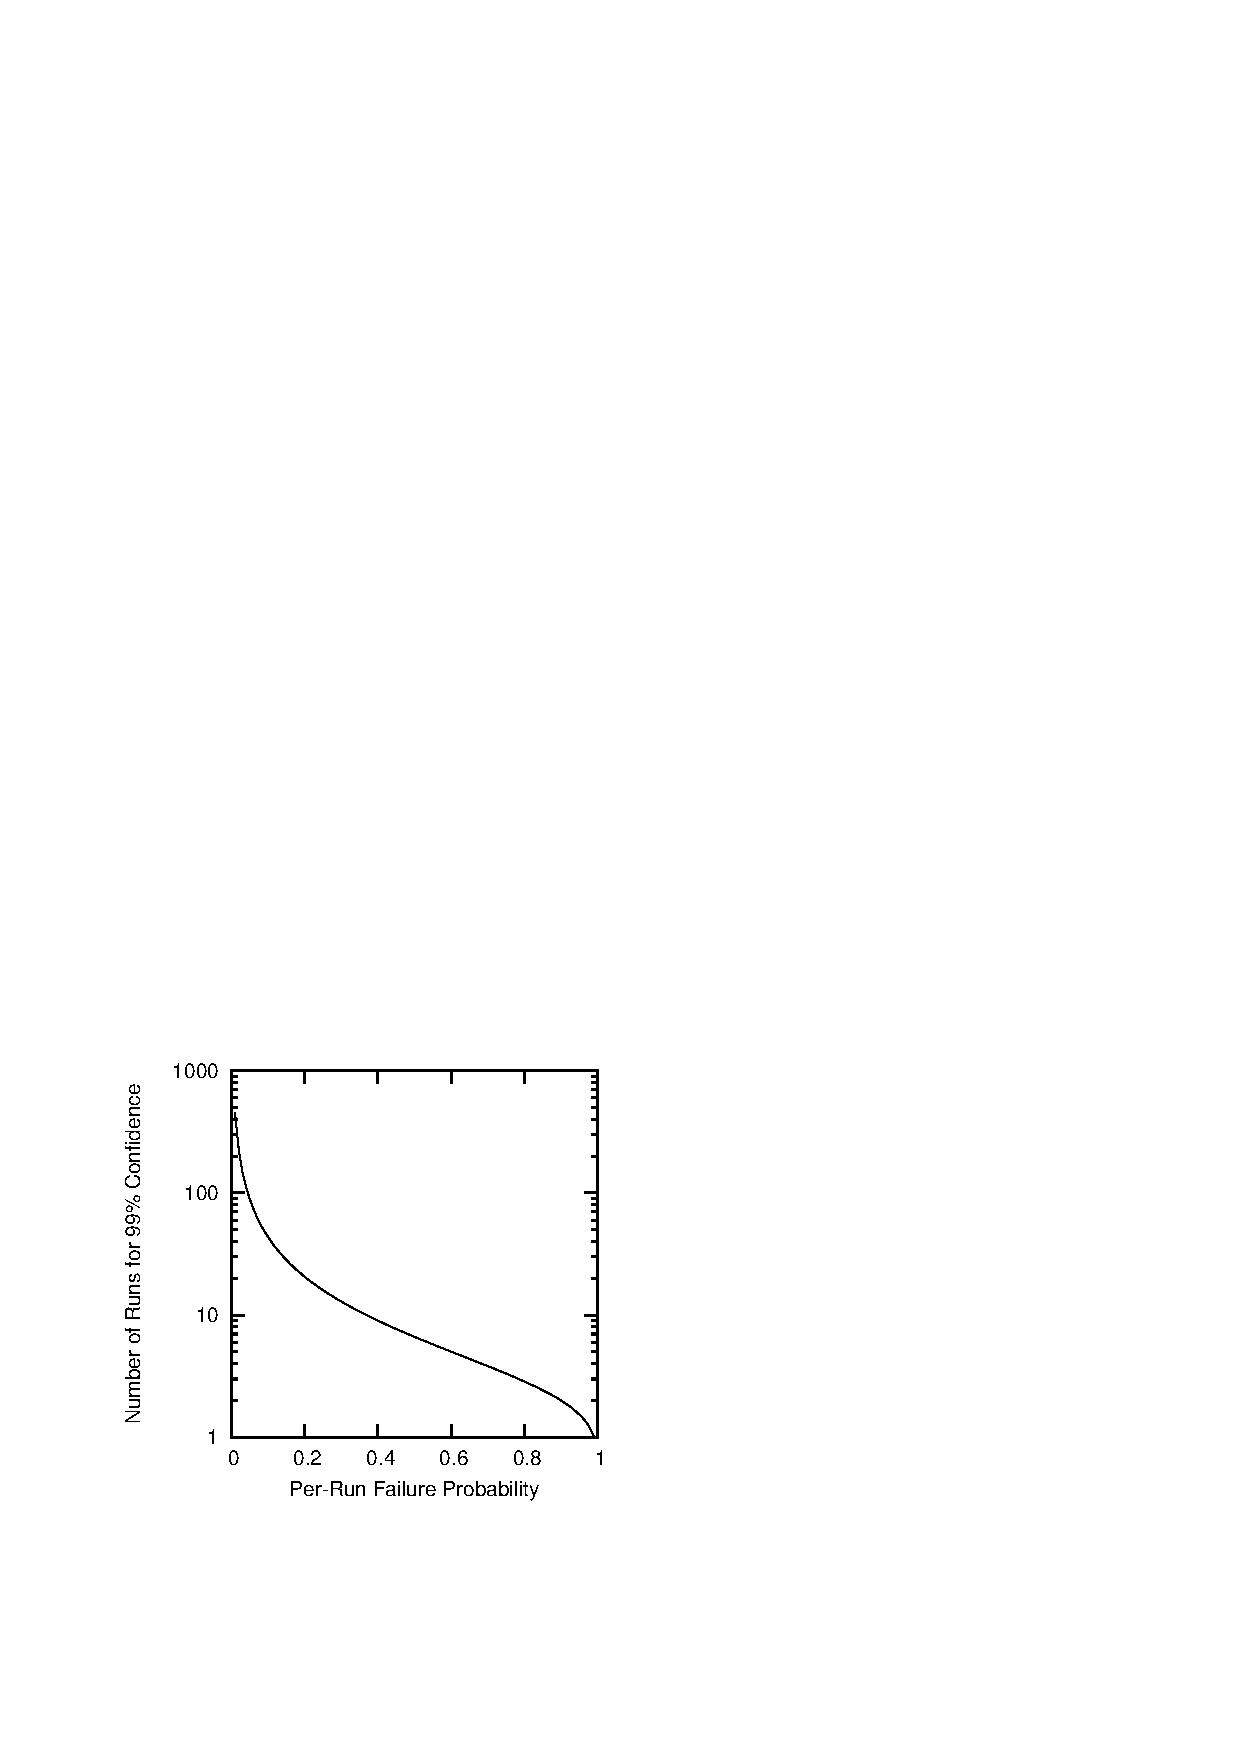
\includegraphics{CodeSamples/debugging/BinomialNRuns}}
\end{center}
\caption{Number of Tests Required for 99 Percent Confidence Given Failure Rate}
\label{fig:debugging:Number of Tests Required for 99 Percent Confidence Given Failure Rate}
\end{figure}

Figure~\ref{fig:debugging:Number of Tests Required for 99 Percent Confidence Given Failure Rate}
shows a plot of this function.
Not surprisingly, the less frequently each test run fails, the more
test runs are required to be 99\% confident that the bug has been
fixed.
If the bug caused the test to fail only 1\% of the time, then a
mind-boggling 458 test runs are required.
As the failure probability decreases, the number of test runs required
increases, going to infinity as the failure probability goes to zero.

The moral of this story is that when you have found a rarely occurring
bug, your testing job will be much easier if you can come up with
a carefully targeted test with a much higher failure rate.
For example, if your targeted test raised the failure rate from 1\%
to 30\%, then the number of runs required for 99\% confidence
would drop from a mind-boggling 458 test runs to a mere thirteen test runs.

But these thirteen test runs would only give you 99\% confidence that
your fix had produced ``some improvement''.
Suppose you instead want to have 99\% confidence that your fix reduced
the failure rate by an order of magnitude.
How many failure-free test runs are required?

An order of magnitude improvement from a 30\% failure rate would be
a 3\% failure rate.
Plugging these numbers into
Equation~\ref{eq:debugging:Binomial Number of Tests Required} yields:

\begin{equation}
	n = \frac{\log\left(1 - 0.99\right)}{\log\left(1 - 0.03\right)} = 151.2
\end{equation}

So our order of magnitude improvement requires roughly an order of
magnitude more testing.
Certainty is impossible, and high probabilities are quite expensive.
Clearly making tests run more quickly and making failures more probable
are essential skills in the development of highly reliable software.
These skills will be covered in a later section.

\subsection{Abusing Statistics for Discrete Testing}
\label{sec:Abusing Statistics for Discrete Testing}

But suppose that you have a continuous test that fails about three
times every ten hours, and that you fix the bug that you believe was
causing the failure.
How long do you have to run this test without failure to be 99\% certain
that you reduced the probability of failure?

Without doing excessive violence to statistics, we could simply
redefine a one-hour run to be a discrete test that has a 30\%
probability of failure.
Then the results of in the previous section tell us that if the test
runs for 13 hours without failure, there is a 99\% probability that
our fix actually improved the program's reliability.

A dogmatic statistician might not approve of this approach, but the
sad fact is that the errors introduced by this sort of abuse of
statistical methodology are usually way down in the noise compared to the
errors inherent in your measurements of your program's failure rates.
Nevertheless, the next section describes a slightly less dodgy approach.

\subsection{Statistics for Continuous Testing}
\label{sec:Statistics for Continuous Testing}

@@@ continuous formulation for time-based tests leads to Poisson distribution.
This can be handled using maxima with \co{quantile_poisson()} and
\co{cdf_poisson()}, after a \co{load(distrib)}.

@@@ Note that when you subdivide the tests, you must decrease the value
as well as the probability to maintain the same mean value.

\subsection{Heisenbugs and Creating Anti-Heisenbugs}
\label{Heisenbugs and Creating Anti-Heisenbugs}

This line of thought also leads to an understanding of heisenbugs:
adding tracing and assertions can easily \emph{reduce} the probability
of a bug appearing.
And this is why extremely lightweight tracing and assertion mechanism are
so critically important.

Measure bug probability as a function of configuration parameters,
input, intensity of load, number of CPUs, etc.
Set up experiments.

\section{Performance Estimation}
\label{sec:analysis:Performance Estimation}

{\em @@@ pull in concepts and methods from
\url{http://www.rdrop.com/users/paulmck/scalability/paper/lockperf_J_DS.2002.05.22b.pdf}.}

\subsection{Profiling}
\label{sec:analysis:Profiling}

\subsection{Differential Profiling}
\label{sec:analysis:Differential Profiling}

{\em @@@ pull in concepts and methods from
\url{http://www.rdrop.com/users/paulmck/scalability/paper/profiling.2002.06.04.pdf}.
Also need tools work.}
